\chapter{Lecture 7 - Charts}
Spatial axes are an important ingredient in visualization. One should always label the axes and set the standard unit of distance between two points in the chart. This layout can be:
\begin{itemize}[noitemsep]
    \item rectilinear: items distributed along two perpendicular axes, with values ranging from a minimum to a maximum. (like in most of the tables mentioned in Chapter 6)
    \item parallel: axes placed parallel to each other (in the case of a slope chart)
    \item radial: items distributed around a circle, using the angle channel (like in a pie chart)
\end{itemize}

\subsubsection{Radial layout}
Items in a radial layout are distributed around a circle, using the angle channel. The most natural coordinate system in radial layout is polar coordinates, where one dimension is measured as an angle from a starting line, and the other dimension is measured as a distance from a center point. Compared to a rectilinear spatial position channel, the angle channel is less accurately perceived.

\section{Radial bar chart}
The radial bar chart is similar to a bar chart, using the same line marks to encode a quantitative attribute with the length channel, the only difference being the radial vs rectilinear orientation of the axes. This chart can be messy to the eye; it is usually a good idea to re-order the bars to that the comparison from the highest to the smallest values can be perceived. This chart can be revisited to encode multiple attributes. 

\begin{figure}[htbp]
    \centering

    \begin{subfigure}[b]{0.4\linewidth}
        \centering
        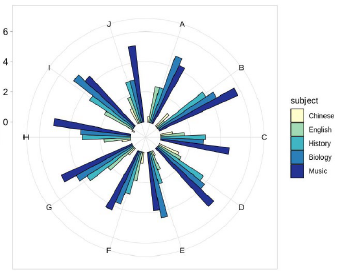
\includegraphics[width=0.5\linewidth]{imgs/lecture7/7.1 radial bar chart.png}
        \caption{encoding multiple attributes}
        \label{fig:7.1a}
    \end{subfigure}
    \hfill
    \begin{subfigure}[b]{0.4\linewidth}
        \centering
        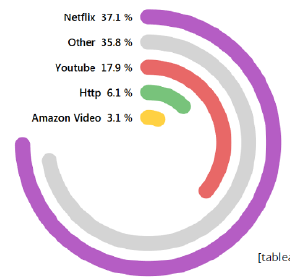
\includegraphics[width=0.5\linewidth]{imgs/lecture7/7.2 radial bar chart.png}
        \caption{different forms of radial bar chart}
        \label{fig:7.2b}
    \end{subfigure}

    \caption{Different use of radial bar chart}
    \label{fig:7.1}
\end{figure}

\subsubsection{Recap: Radial bar chart}
\begin{tabularx}{0.8\textwidth} { 
  | >{\raggedright\arraybackslash}l 
  | >{\raggedright\arraybackslash}X | }
    \hline
    Data (What) & Table with one quantitative value attribute and one categorical key attribute \\
    \hline
    Encode (How) & Length coding of line marks, radial layout \\
    \hline
\end{tabularx}

\section{Pie chart}
The pie chart is the most commonly used radial graphic; it uses 2D area marks and the angle (arc length) channel. It is used to show percentages and proportions among categories by dividing a circle into proportional segments, with each angle/arc length representing the value/proportion for each category, and the full circle represents the sum of all data, i.e., 100\%. \par
Despite the popularity, pie charts are clearly problematic when considered according to the visual channel properties. While it is useful for giving a quick idea and to compare one slice against the total, it is not good for an accurate comparison: angle judgments on area marks are less accurate than length judgments on line marks; the wedges vary in width along the radial axis, from narrow near the center to wide near the end, making the area judgments difficult. In addition, scalability is an issue; it can shows up to tens of categories, simply because as the number of categories increases, the size of each segment decreases, not to mention the size of the legend would also become proportionally large. \par
The most useful property of pie charts is that they show the relative contribution of parts to a whole; however, this property is unique to pie charts. A single bar in a normalized stacked bar chart would do the same job with a more accurate channel of length.\par
A pie chart is also one of the most commonly \textit{misused} visualization:
\begin{itemize}[noitemsep]
    \item sum of the percentage of all slices differ from 100\%
    \item redundant representations of data (sometimes people would put a number, a percentage of the slice to the whole, together with the slice)
    \item unnecessary and unjustified channel, like 3D (applies to all types to visualization)
    \item incomplete pie chart showing only some slices, \textit{but}, depending on the context, it can be useful for emphasizing the portion on the given topic, thus, showing comparison between different subjects.
\end{itemize}

\begin{figure}[htbp]
    \centering
    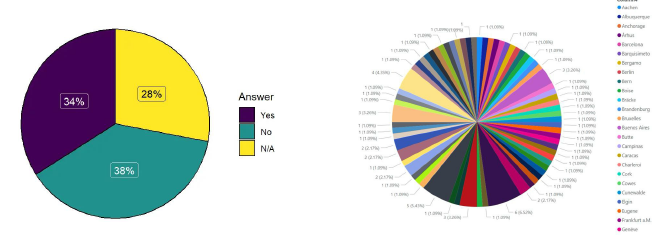
\includegraphics[width=0.5\linewidth]{imgs/lecture7/7.3 pie chart misuse.png}
    \caption{Pie chart misuses}
    \label{fig:7.2}
\end{figure}

\subsubsection{Donut chart}
It is a variant of a pie chart with the center area cut out, making the focus on arc length rather than on area. It is more efficient on space occupancy while providing more space for labels.

\subsubsection{Polar area chart}
Another variation of a pie chart that varies the length of the wedge, rather than varying angles. 

\subsubsection{Radar chart}
Also called a spider chart or star chart, where items are displayed along circles, it is useful for periodic data. This chart can easily compare properties of a class of objects or a category, but not as much in understanding the trade-off between variables. One should be careful when using it for many variables or many data points.

\subsubsection{Sunburst chart}
It has a radial layout but can be used to visualize hierarchies. A sunburst chart visualizes hierarchies (a tree structure) with concentric circles where each ring represents a level in the hierarchy, moving outwards. \par
It used multiple channels, such as distances from the center representing levels in the hierarchy, the angle representing connections among items (nodes), and color can also give additional information about the items. Note that each ring does not have to be complete, as a tree does not have to be perfectly balanced.

\begin{figure}[htbp]
    \centering
    
    % First row (3 images)
    \begin{subfigure}{0.45\textwidth}
        \centering
        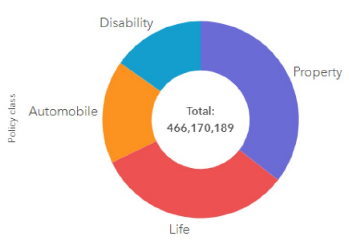
\includegraphics[width=0.7\linewidth]{imgs/lecture7/7.4 donut chart.png}
        \caption{Donut chart}
        \label{fig:7.3a}
    \end{subfigure}
    \hfill
    \begin{subfigure}{0.45\textwidth}
        \centering
        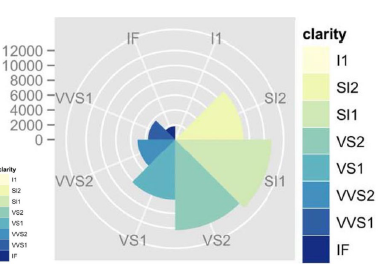
\includegraphics[width=0.7\linewidth]{imgs/lecture7/7.5 polar area chart.png}
        \caption{Polar area chart}
        \label{fig:7.3b}
    \end{subfigure}

    \vspace{0.5cm}

    % Second row (2 images)
    \begin{subfigure}{0.45\textwidth}
        \centering
        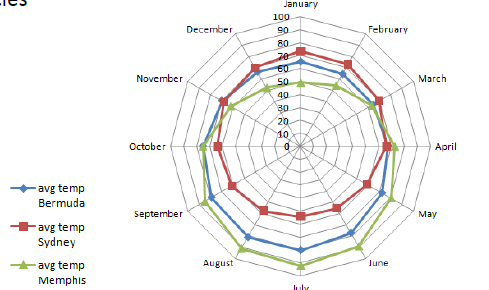
\includegraphics[width=0.7\linewidth]{imgs/lecture7/7.6 spider chart.png}
        \caption{Radar chart (or spider chart)}
        \label{fig:7.3c}
    \end{subfigure}
    \hfill
    \begin{subfigure}{0.45\textwidth}
        \centering
        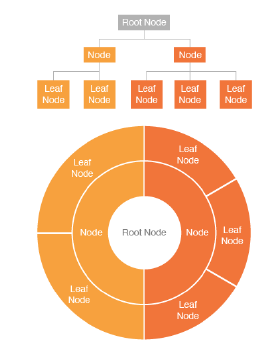
\includegraphics[width=0.7\linewidth]{imgs/lecture7/7.7 sunburst chart.png}
        \caption{Sunburst chart}
        \label{fig:7.3d}
    \end{subfigure}

    \caption{Variations of a pie chart}
    \label{fig:7.3}
\end{figure}

\section{Treemap}
A treemap is an alternative way to visualize hierarchies, by displaying quantities via area size. Each rectangle represents a category, with nested subcategory rectangles. Child nodes are contained in the area region representing the parent node. When a quantity is assigned to a category, its area size is displayed in proportion to that quantity and to the other quantities within the same parent category in a part-to-whole relationship.\par
The treemap is very compact and space-efficient, but it is not as good as a sunburst chart in showing the levels in the hierarchy, because only leaf attributes are displayed. In general, it is a good option for showing the overall structure and providing an estimated comparison via area sizes.

\subsubsection{Bubble hierarchy}
As with a treemap, it uses containment to represent hierarchies and area to visualize quantities, but with bubbles-shaped containers rather than rectangles. 

\begin{figure}[htbp]
    \centering
    
    \begin{subfigure}{0.45\textwidth}
        \centering
        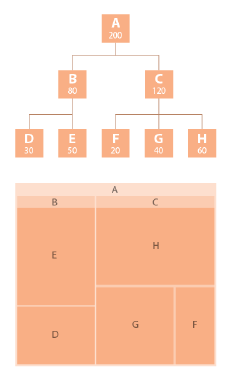
\includegraphics[width=0.6\linewidth]{imgs/lecture7/7.8 treemap.png}
        \caption{Treemap}
        \label{fig:7.4a}
    \end{subfigure}
    \hfill
    \begin{subfigure}{0.45\textwidth}
        \centering
        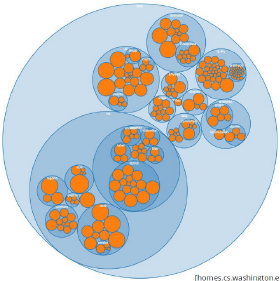
\includegraphics[width=0.5\linewidth]{imgs/lecture7/7.9 bubble hierarchy.png}
        \caption{Bubble hierarchy}
        \label{fig:7.4b}
    \end{subfigure}

    \caption{Treemap and Bubble hierarchy variant}
    \label{fig:7.4}
\end{figure}

\subsection{Different representations of a tree dataset}
\begin{figure}[htbp]
    \centering
    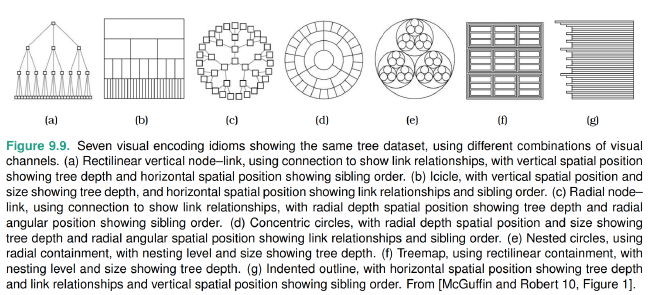
\includegraphics[width=0.88\linewidth]{imgs/lecture7/7.10 visualizing a tree.png}
    \caption{Visualizing a tree dataset}
    \label{fig:7.5}
\end{figure}